\section{Detector Calibration}
\label{sec:calibration}
Calibration is extremely important to translating the response of the detector into the actually physical properties of an observed process.  The response of the SK detector to a particular physics process is essentially the combination of three responses:
\begin{itemize}
\item The physics of the initial process and production of photons through Cherenkov radiation
\item The propagation of photons through the water to the PMTs (water transparency)
\item  The response of the PMTs and electronics to the incident photons
\end{itemize}
Since the first response is what we are actually interested in observing, calibration is necessary to understand the second and third responses, so that we can translate the full detector response into an understanding of the actual physics process we are observing.  In this section I will discuss the main components of understanding the second two responses.  A detailed description of these and other aspects of detector calibration can be found in \cite{Abe:2013gga}.

\subsection{Water Transparency}
The propagation of photons through water is dictated by the equation:
\begin{equation}
I(l,\lambda)=I_0(\lambda)e^{\frac{l}{L(\lambda)}}
\label{eq:light_intensity}
\end{equation} 
 where $I(l,\lambda)$ is the intensity of light of wavelength $\lambda$ a distance $l$ from the source, $I_0(\lambda)$ is the initial intensity of the light, and $L(\lambda)$ is the total attenuation length at the given wavelength, which includes both scattering and absorption.  The attenuation length can be broken into three components:
\begin{equation}
L(\lambda)=\frac{1}{\alpha_{abs}(\lambda)+\alpha_{sym}(\lambda)+\alpha_{asy}(\lambda)}.
\end{equation}
Here $\alpha_{abs}(\lambda)$ is the absorption amplitude, $\alpha_{sym}(\lambda)$ is the ``symmetric" scattering amplitude, which is composed of Rayleigh scattering and symmetric Mie scattering, and $\alpha_{asy}(\lambda)$ is the ``asymmetric" scattering amplitude, which is composed of forward Mie scattering.  In order to measure these amplitudes, a collimated laser is injected at a few different wavelengths downward into the SK detector, as show in \cref{fig:laser}.  The detector is divided into seven regions, (top, bottom, five barrel regions), and the absorption and scattering amplitudes are tuned in MC so that the distribution of hits as a function a time in MC agrees with what is seen in data.  The results at the different wavelengths are then used to fit the amplitudes as a function of wavelength to  predetermined polynomial forms.  The results of these fits from a typical calibration run are shown in \cref{fig:water_transparency_results}.

\begin{figure}
\centering
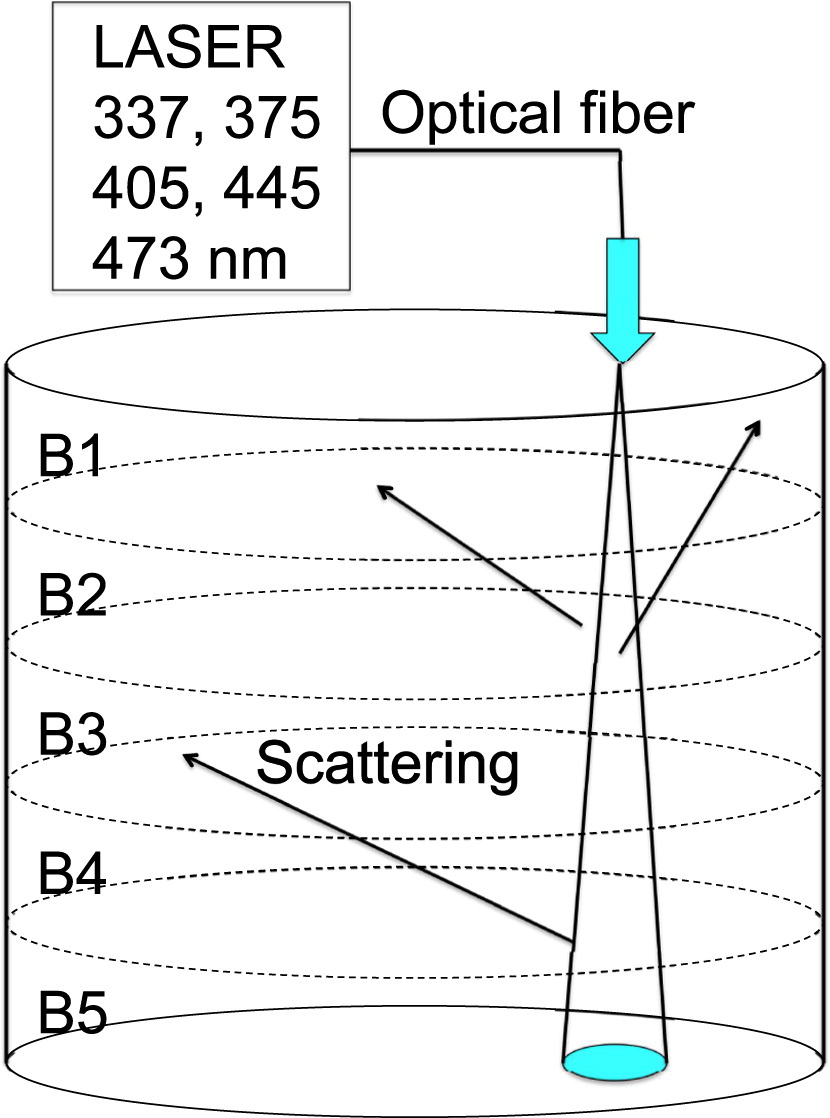
\includegraphics[width=0.5\textwidth]{figures/Laser.jpg}
\caption{Laser setup for water transparency measurement \cite{Abe:2013gga}.}
\label{fig:laser}
\end{figure}

\begin{figure}
\centering
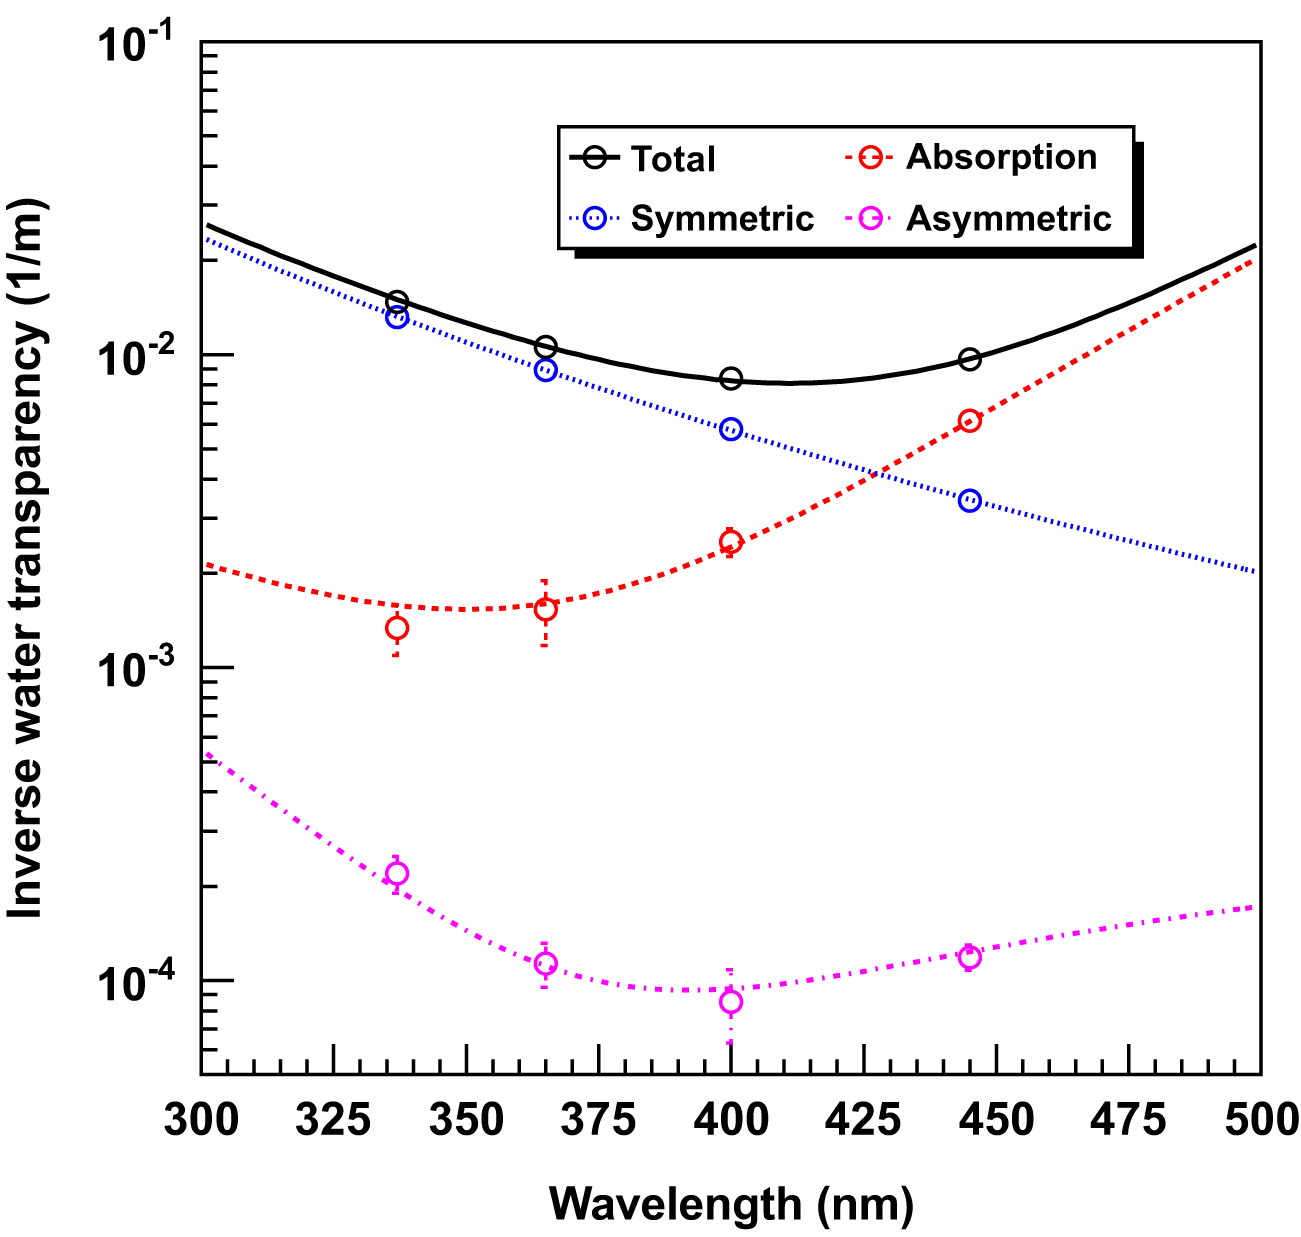
\includegraphics[width=0.5\textwidth]{figures/Water_transperency.png}
\caption{Absorption amplitude results from a typical laser calibration run \cite{Abe:2013gga}.}
\label{fig:water_transparency_results}
\end{figure}

\subsection{PMT and Electronics Response}
When light hits a PMT, a voltage pulse is produced by the PMT.  The actual information recorded by the SK electronics is the charge of the pulse, and the time the rising edge of the pulse crossed a discriminator threshold.  In order to correctly simulate how a certain number of photons at a particular time will be translated into an electronics response, calibration of the PMTs and SK electronics is required.\par
\subsection{Charge Response}
First, the high voltage (HV) for each PMT was set so that each PMT would produce the same amount of charge from the same intensity of light.  To do this, 420 ``reference" PMTs were calibrated in a dedicated pre-calibration system before their installation, so that their desired HV settings were known \cite{Abe:2013gga}.  These 420 PMTs were then arranged in the detector in order to take advantage of the cylindrical symmetry of the detector, as shown in \cref{fig:reference_pmts}.  For a light source on the central axis of the detector, the intensity of light at any PMT could be estimated by the response of the reference PMTs with the same geometric relationship to the light source.  A Xe-lamp fed into a scintillator ball which resulted in isotropic light was used as the light source in both the pre-calibration of the 420 reference PMTs and in the calibration of all the PMTs in the tank. \par
\begin{figure}
\centering
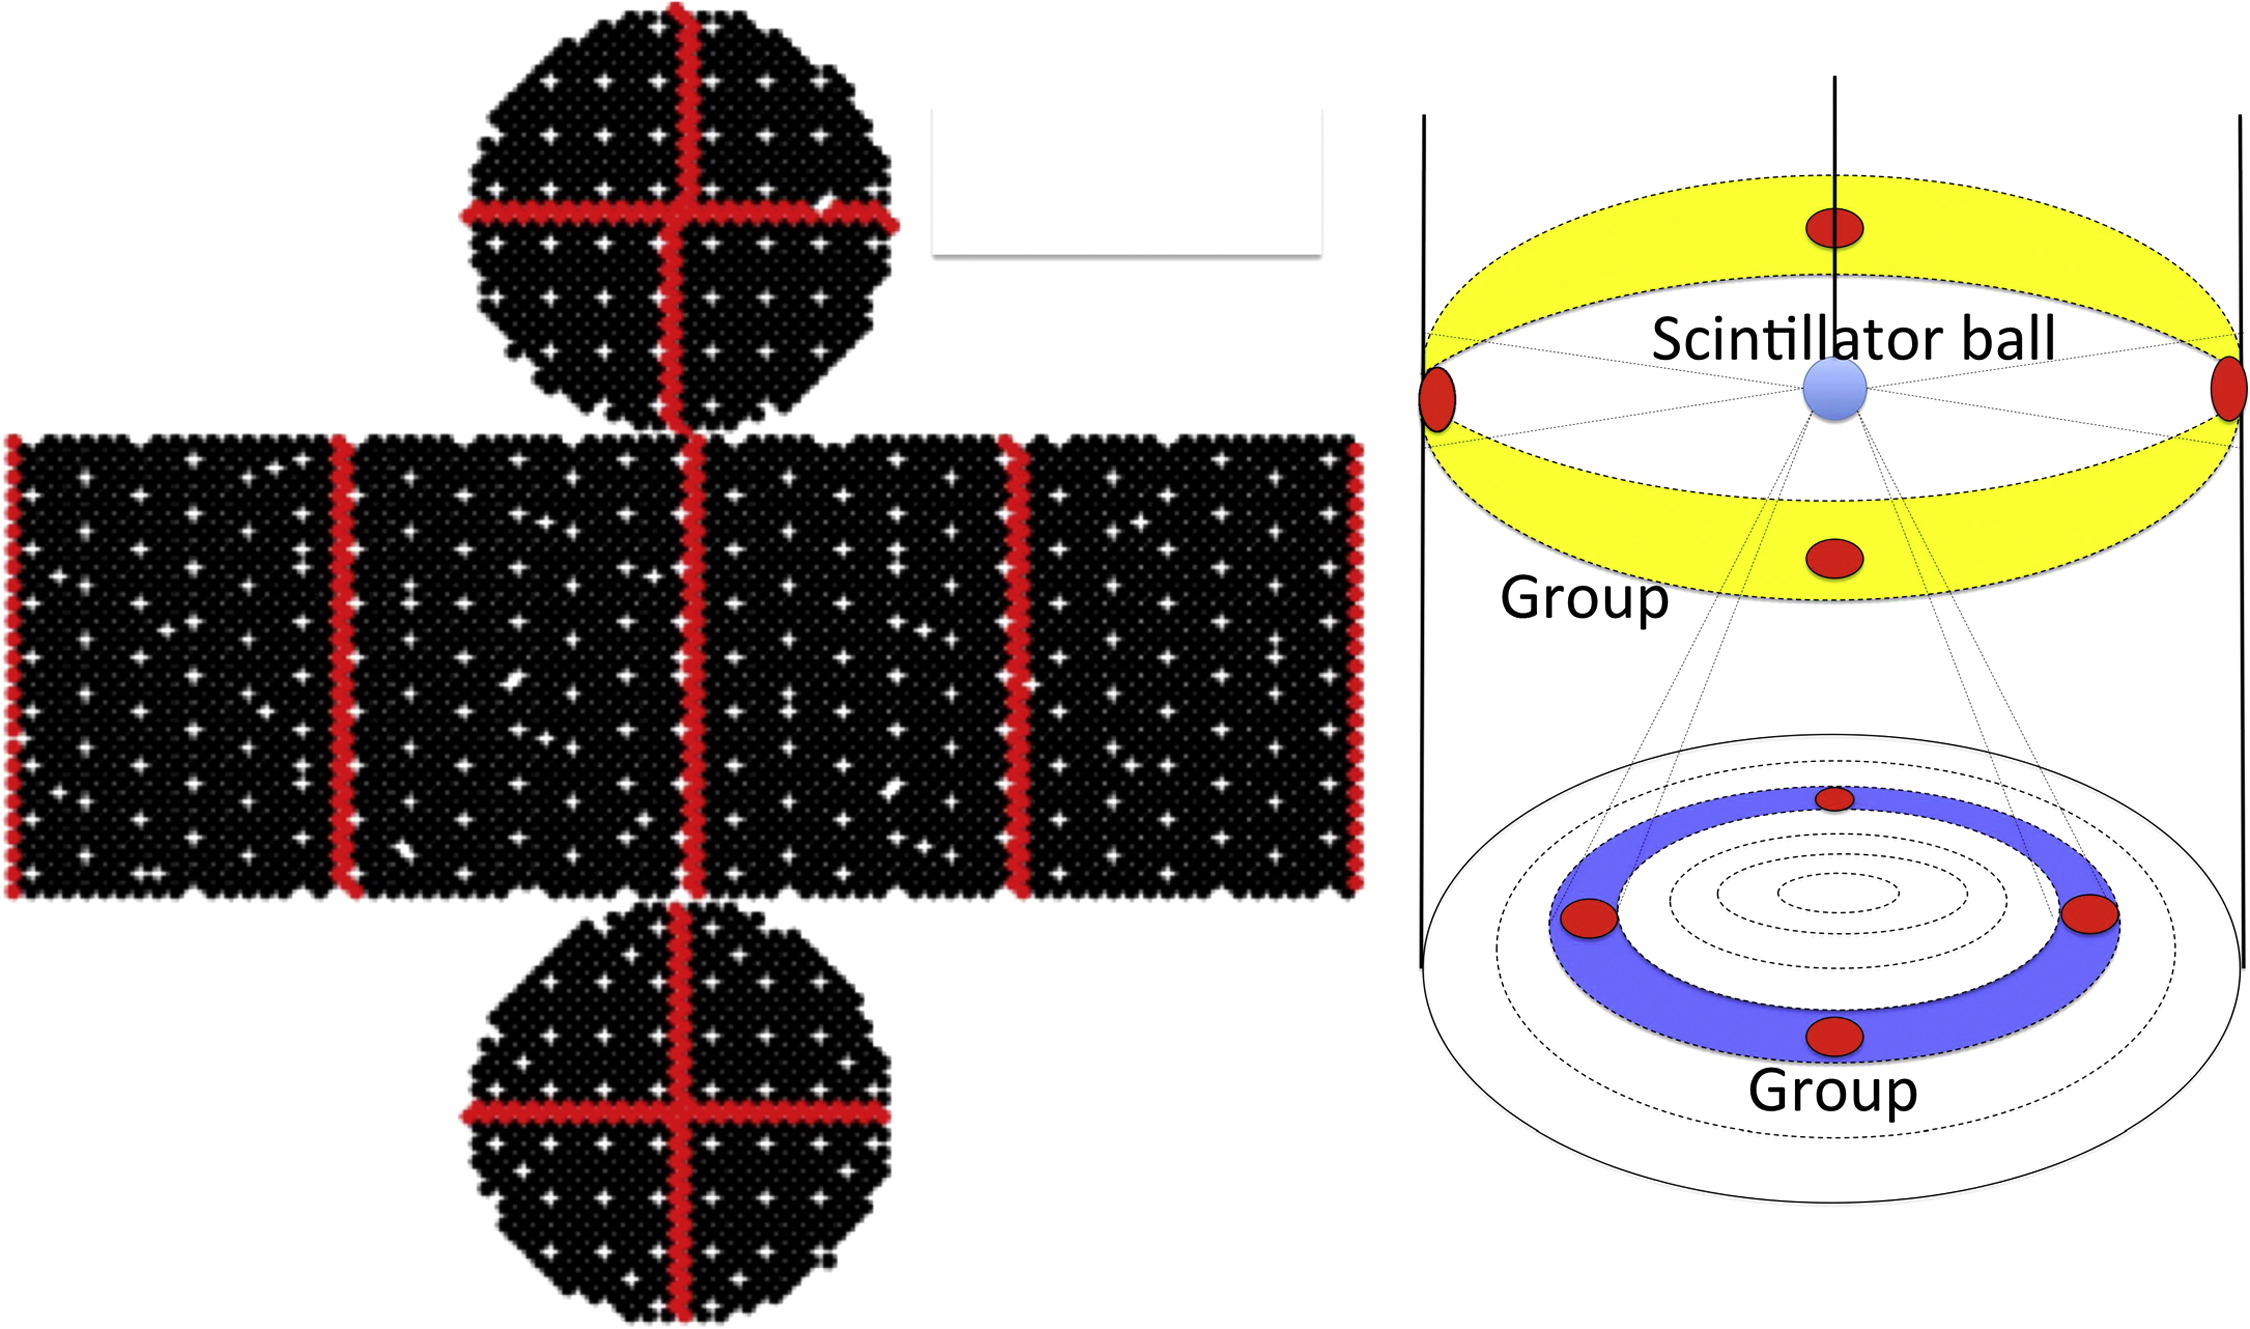
\includegraphics[width=0.8\textwidth,keepaspectratio]{figures/reference_pmts.png}
\caption{Location of the 420 reference PMTs used for HV calibration \cite{Abe:2013gga}.}
\label{fig:reference_pmts}	
\end{figure}  

Once the HV setting for each PMT has been assigned, the expected charge from incident light of intensity $I$ on the $i^{th}$ PMT can be written as:
\begin{equation}
Q_i=I \times QE_i \times G_i
\label{eq:expected_charge}
\end{equation}
where $QE_i$ and $G_i$ are the quantum efficiency and gain of the $i^{th}$ PMT.  Simulation of PMT response thus require the measurement of quantum efficiency and gain for each PMT.  \par
Gain calibration is performed first, and this is done in two steps.  In the first step, the relative gain of each PMT compared to the average is calculated.  Then the absolute gain of the full detector is found.  Between these two measurements, the absolute gain of each individual PMT can be found as well.  \par
The relative gain measurement is performed as follows.  A stable light source which emits constant amplitude flashes is placed in the detector and run in two different modes.  In the first mode, the source produces high-intensity flashes, so that each PMT observes a reasonable number of photons.  In this mode, the average charge observed by PMT $i$ can be written as 
\begin{equation}
Q_{obs}(i) \propto I_{high} \times a_i \times QE_i \times G_i
\end{equation}  
where $I_{high}$ is the intensity of the light source in the high-intensity setting and $a_i$ is the acceptance of the $i^{th}$ PMT, which accounts for water transparency and geometrical affects.  In the second mode, the light source produces low-intensity flashes, so that hits on PMTs can be assumed to be only single photo-electrons (pe's).  In this mode, the number of hits when the charge crosses a threshold value can be written as 
\begin{equation}
N_{obs}(i)\propto I_{low} \times a_i \times QE_i.
\end{equation}
Note that in this mode, the number of hits is mostly independent of gain.  In this way, the relative gain for each PMT can be extracted as 
\begin{equation}
G_i \propto \frac{Q_{obs}(i)}{N_{obs}(i)}
\end{equation}
where the proportionality constant is the same for all PMTs.  The distribution of relative gains is shown in \cref{fig:relative_gain}, with the average gain normalized to 1.\par
\begin{figure}
\centering
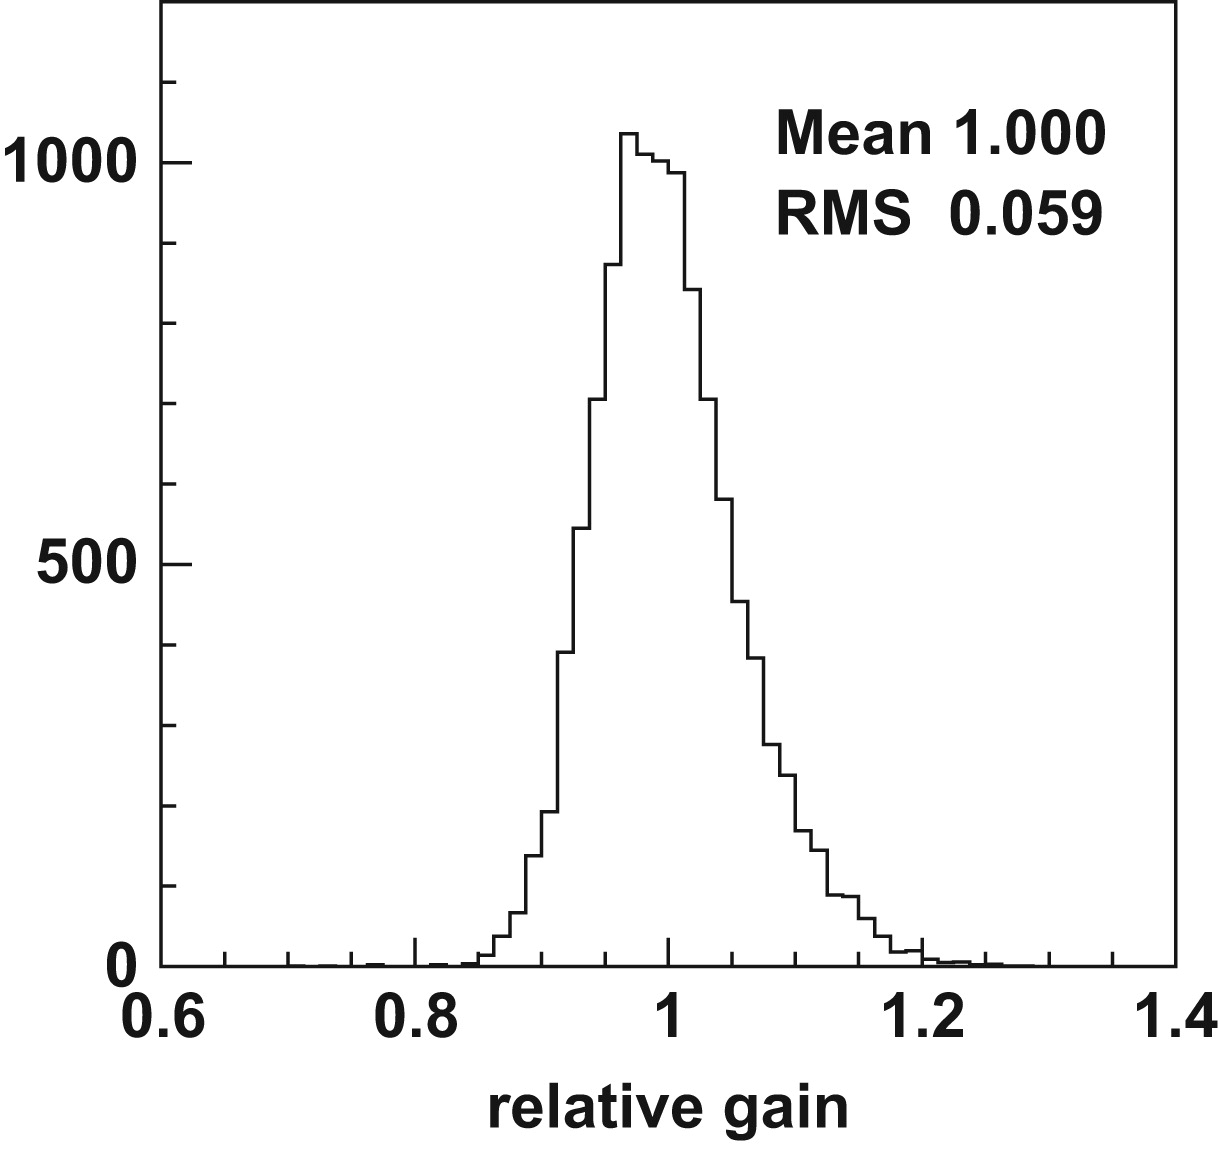
\includegraphics[width=0.5\textwidth,keepaspectratio]{figures/relative_gain.png}
\caption{Distribution of relative gains of PMTs \cite{Abe:2013gga}.}
\label{fig:relative_gain}	
\end{figure} 
With the relative gains of each PMT known, a nickel source which produces gamma-rays isotropically is placed in the detector.  The source is faint enough that over 99\% of observed PMT hits come from single pe.  The charge of the resulting pulses are corrected by the relative gains for each PMT, and the single PMT distribution of the entire detector is thus found.  This distribution is shown as measured during SK-III is shown in \cref{fig:single_pe}.\par
\begin{figure}
\centering
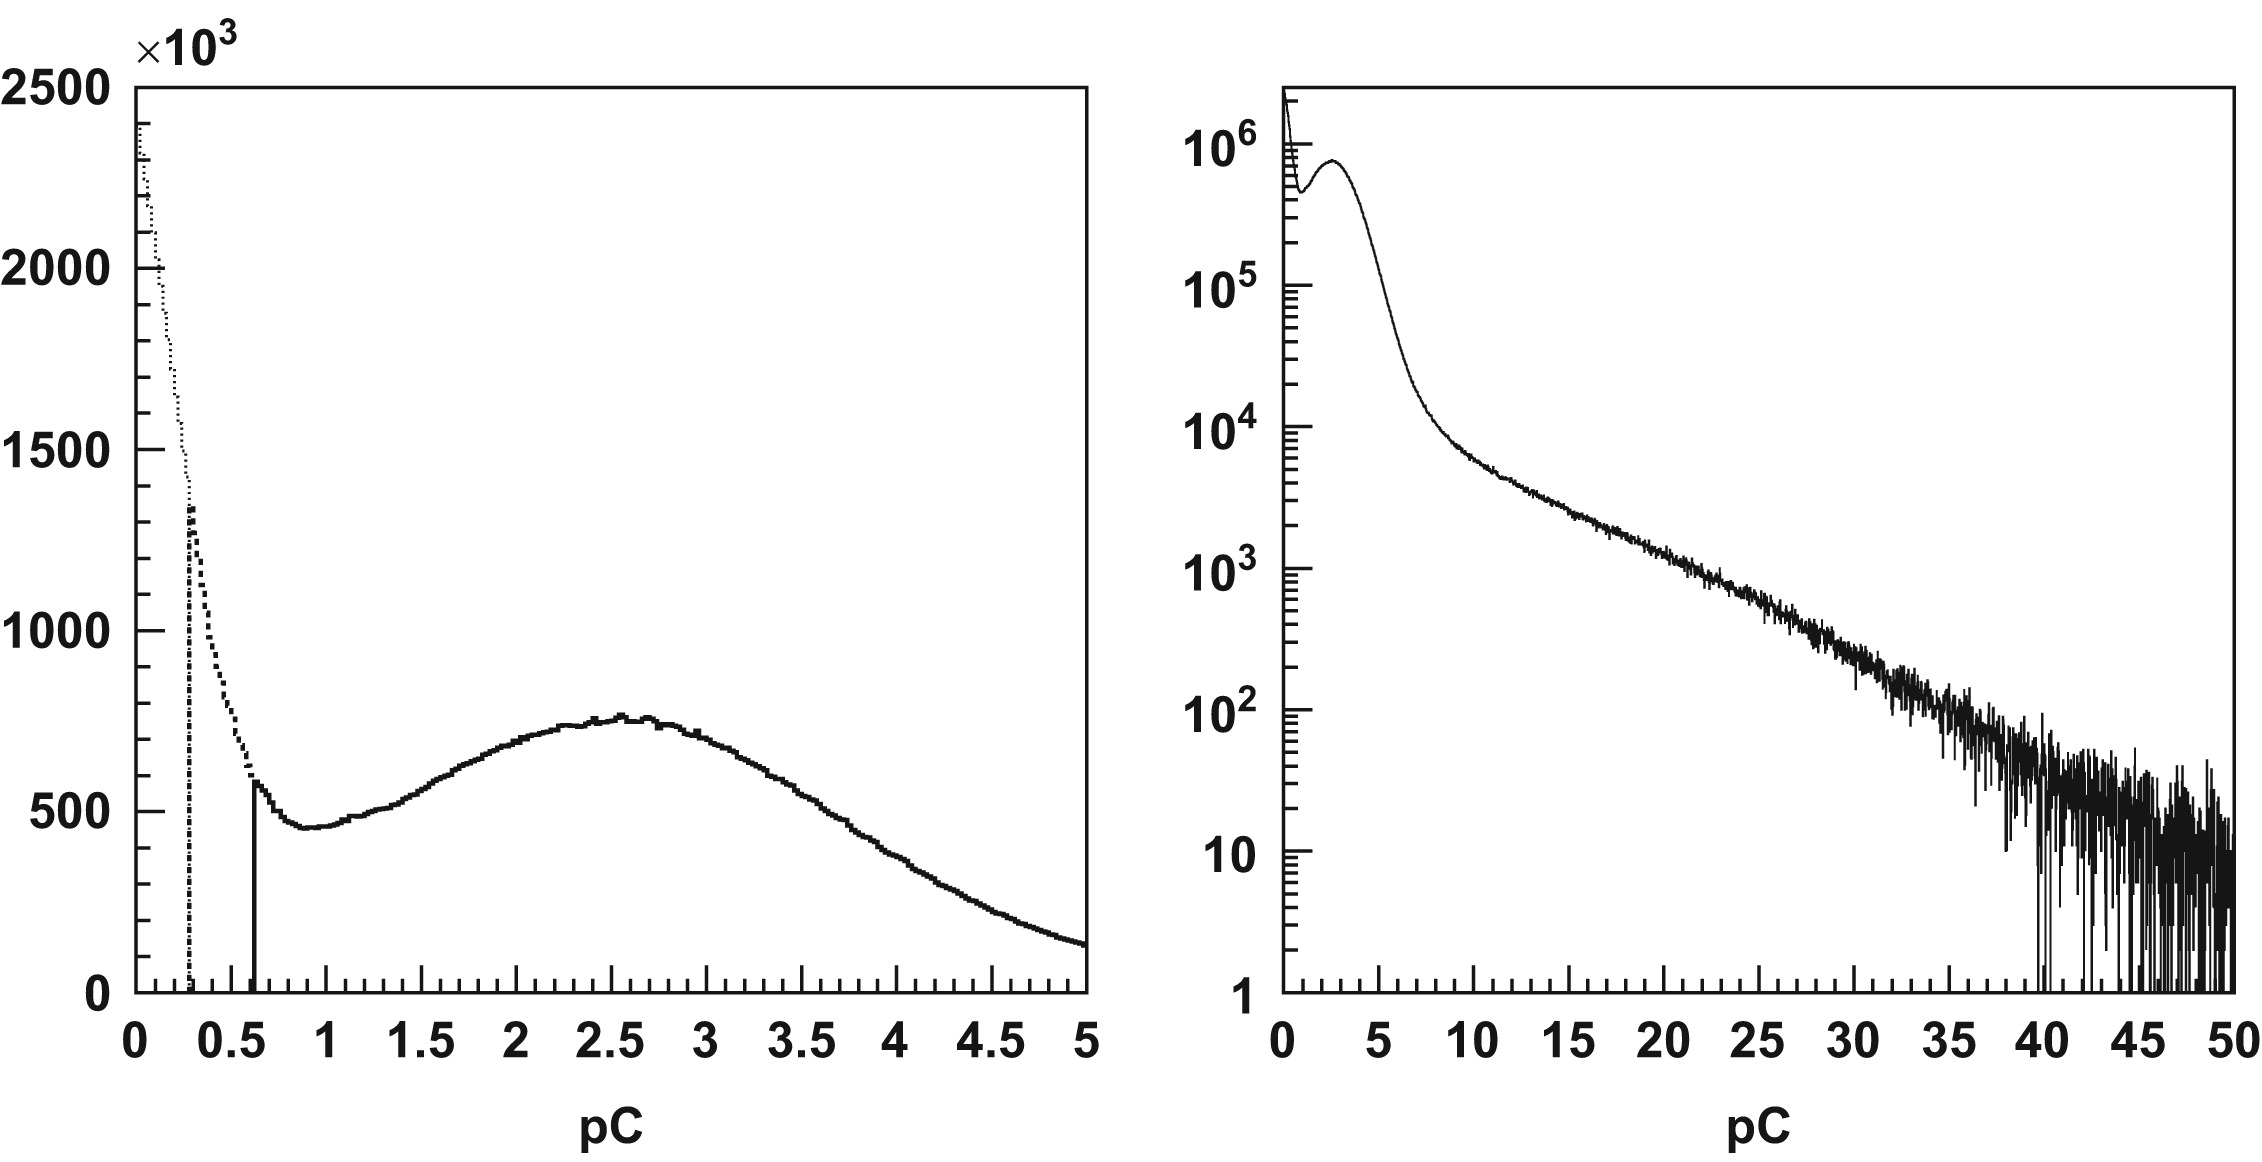
\includegraphics[width=0.8\textwidth,keepaspectratio]{figures/single_pe.png}
\caption{Single pe distribution as measured during SK-III.  The figure on the right shows the same data as on the left, just with a log scale \cite{Abe:2013gga}.}
\label{fig:single_pe}	
\end{figure}
The quantum efficiency of each PMT was found by comparing the number of single-pe hits in a nickel source run to that expected by MC simulation.  The QE in the MC was adjusted until the simulation matched the data well.\par
The response of the PMTs and electronics was also tested by injecting laser light at 30 different intensities into the ID.  This response is shown in \cref{fig:pmt_linearity}, and is used in MC simulation.  \par 
\begin{figure}
\centering
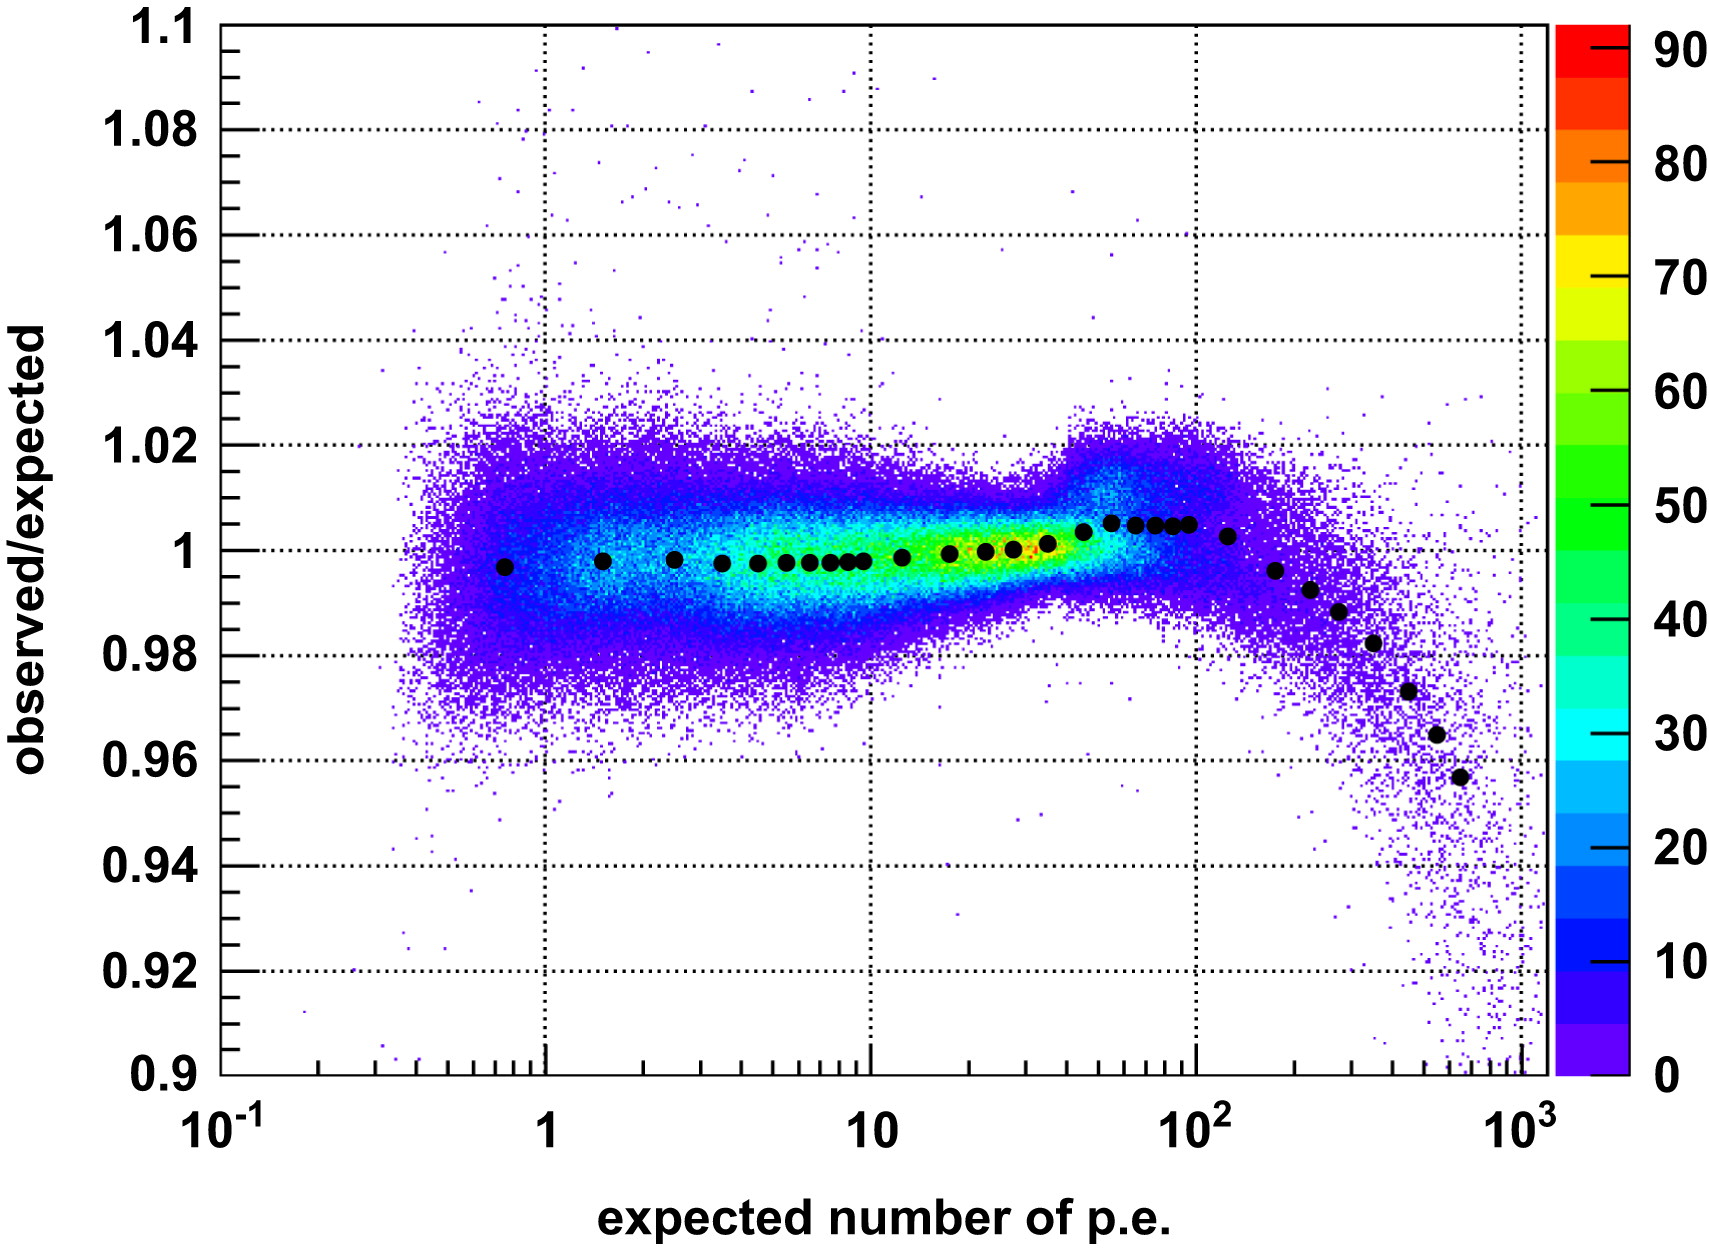
\includegraphics[width=0.5\textwidth,keepaspectratio]{figures/PMT_linearity.png}
\caption{PMT response linearity \cite{Abe:2013gga}.}
\label{fig:pmt_linearity}	
\end{figure} 
\subsection{Timing Response}
The corresponds between the time when a photon hits a PMT and the time when the PMT pulse crosses the discriminator threshold is effected by PMT transit time, cable lengths, and electronics readout time.  Additionally, larger pulses will cross the discriminator threshold faster, and so appear to be earlier hits than smaller pulses.  This is known as "time-walk".  All of these effects must be accounted for by calibration. \par
A nitrogen laser is used to preform timing calibration.  The laser produces fast pulses of light with 0.4 ns FWHM.  These pulses are monitored by a fast response PMT, which defines the time of the pulse.  The laser light is wavelength shifted to 398 nm, and injected in a diffuser ball in the center of the SK tank, which results in isotropic light.  A variable optical filter is used to vary the intensity of the light.\par
During these laser runs, hits in ID PMTs are time-of-flight (TOF) subtracted based on the location of the diffuser ball to account for the time for the light to travel from the diffuser ball tor the particular PMT.  These "residual" times are then compared to the reference time of the laser pulse, based on the monitor PMT.  This comparison gives a conversion between the time that the PMT pulse crosses the discriminator threshold and the time the light actually hit the PMT.  To account for time-walk, this comparison is done as a function of the charge recorded by the PMT, and is called a "TQ-map".  An example TQ-map for a PMT is shown in 
\begin{figure}
\centering
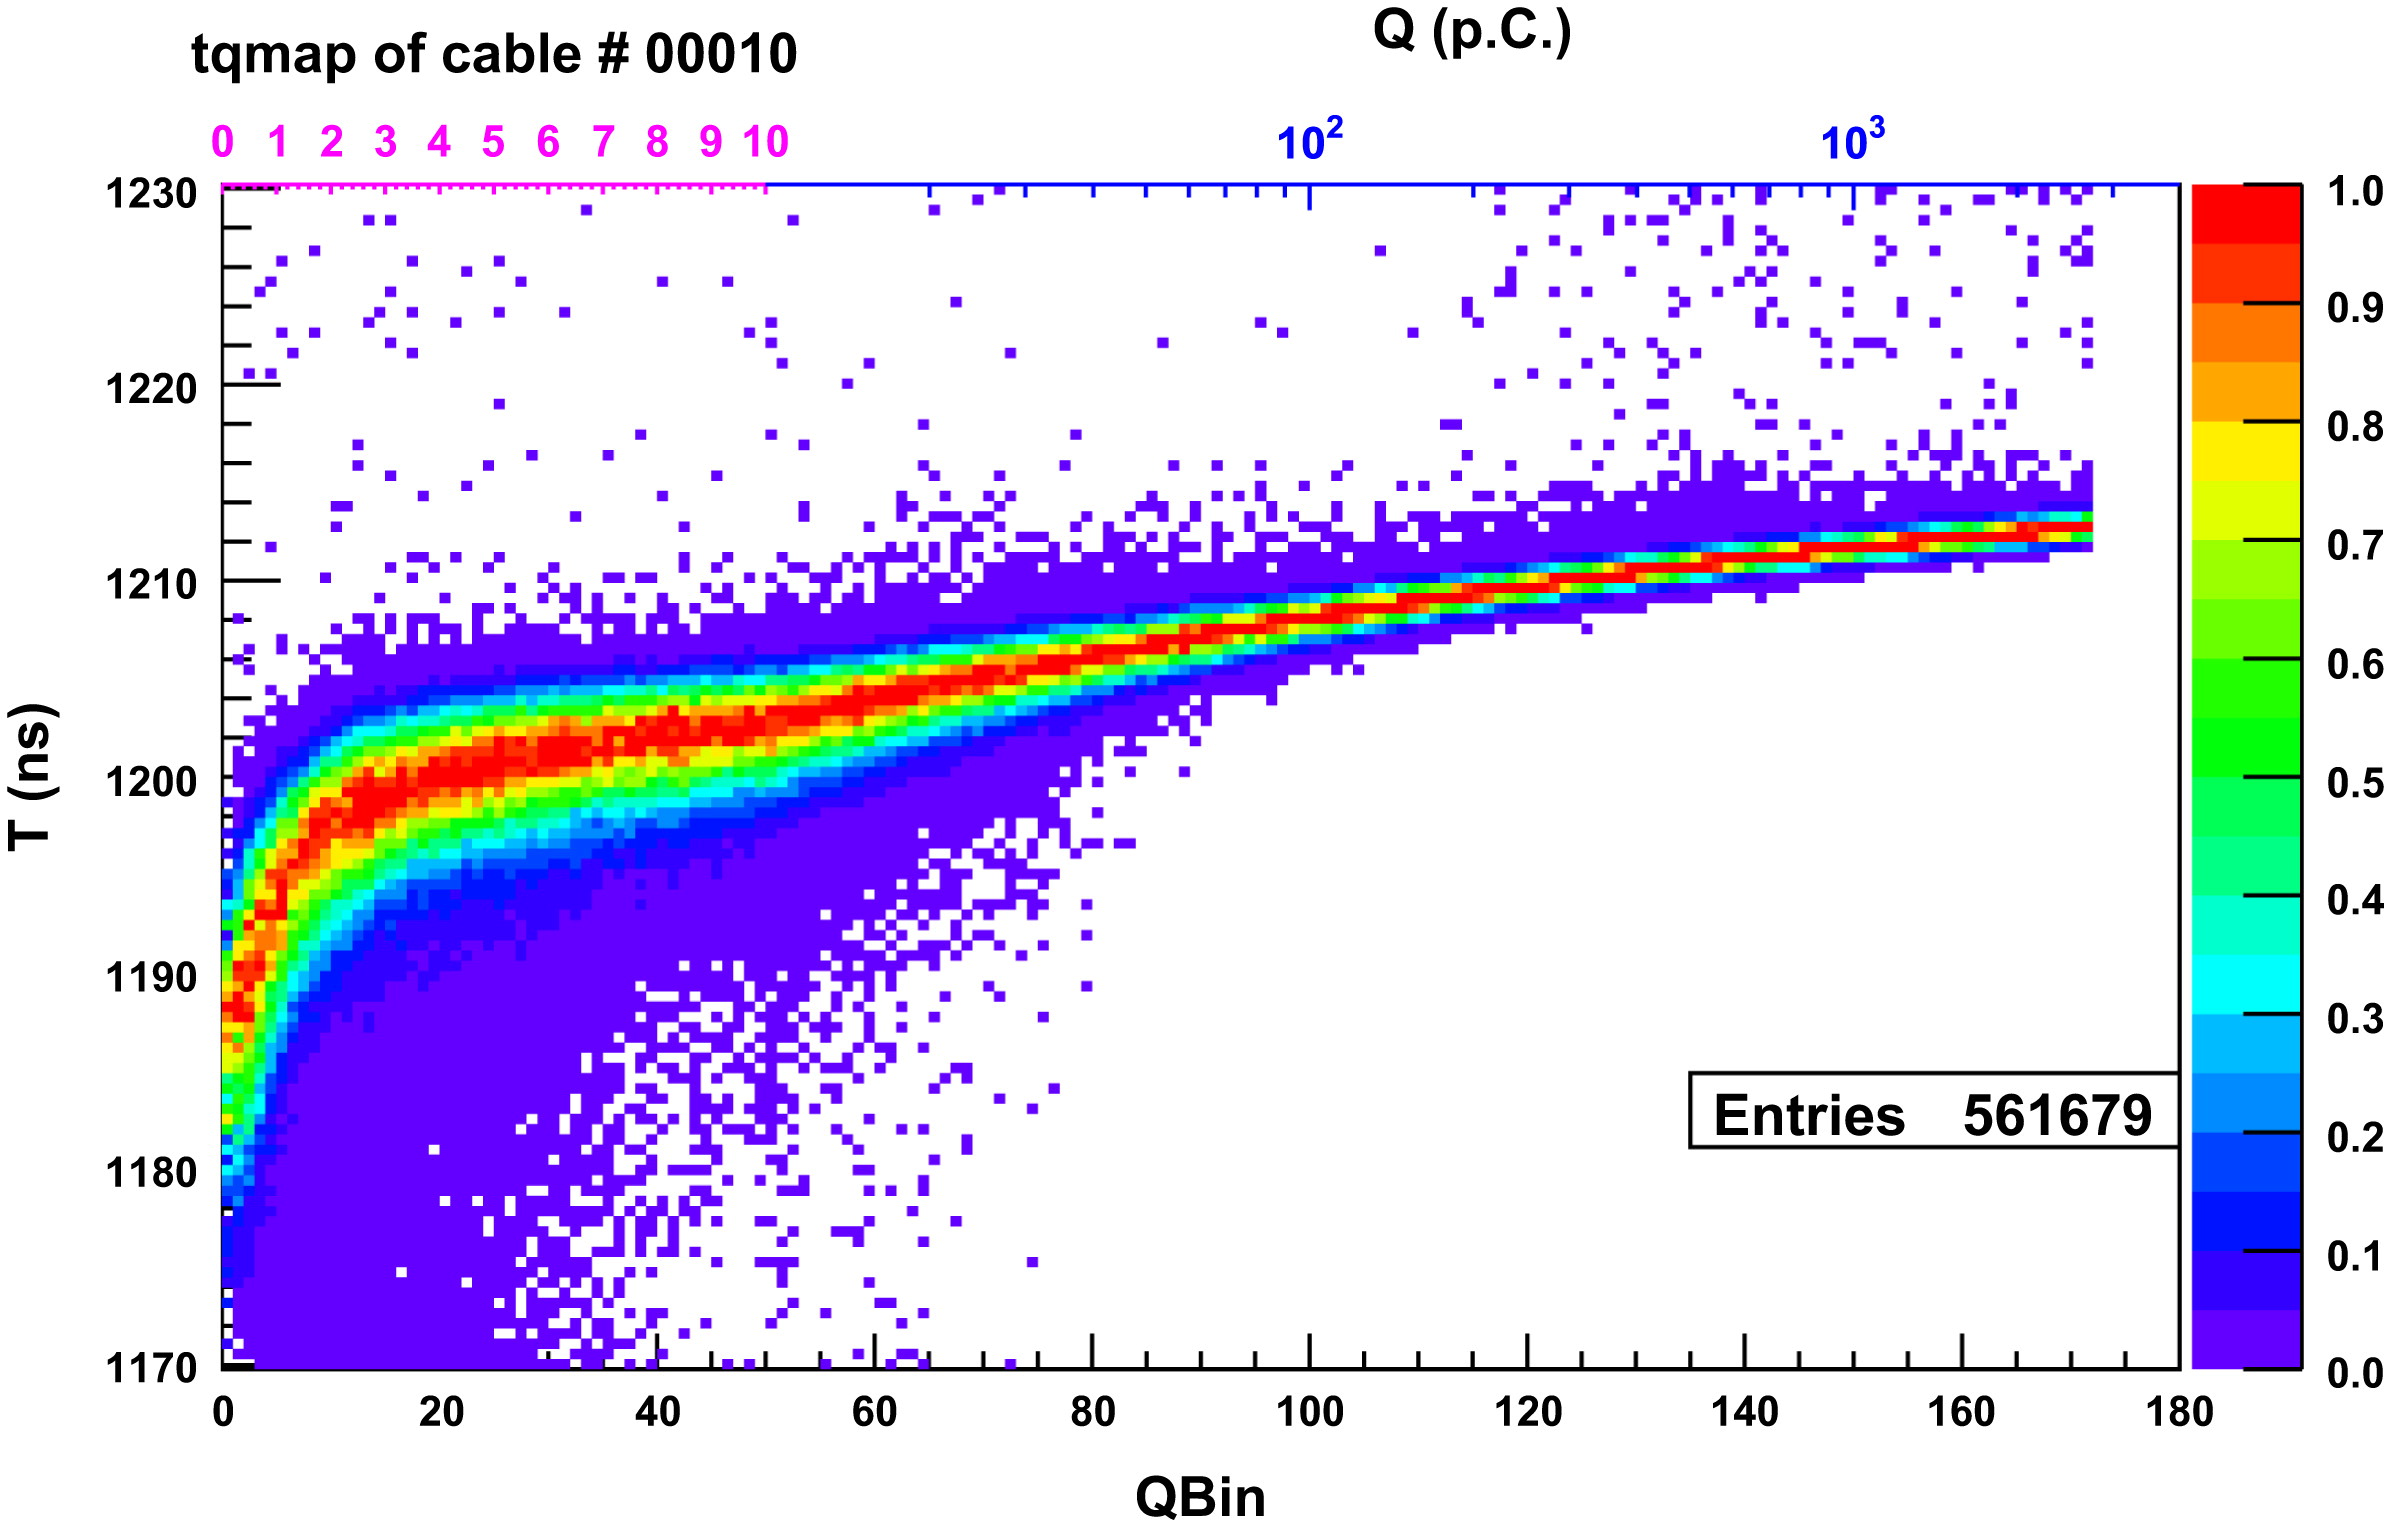
\includegraphics[width=0.5\textwidth,keepaspectratio]{figures/TQ_map.png}
\caption{TQ-map for a PMT.  In this figure larger T corresponds to earlier times, while smaller T corresponds to later times \cite{Abe:2013gga}.}
\label{fig:pmt_linearity}	
\end{figure} 